\chapter{Навчання без учителя.}

Навчання без учителя (Unsupervised Learning) - набір алгоритмів машинного навчання, в яких модель навчається без зазделегідь відомих правильних відповідей. Модель отримує лише набір даних, і намагається самостійно знайти в цих даних приховані закономірності.

Найважливішими задачами навчання без учителя є:

\begin{itemize}
\item кластеризація — автоматичний поділ об'єктів на групи;
\item зменшення розмірності — скорочення кількості ознак без суттєвої втрати інформації;
\item виявлення аномалій — пошук незвичайних або підозрілих об'єктів;
\item аналіз асоціативних правил — пошук закономірностей між подіями або товарами.
\end{itemize}

Ці методи широко застосовуються для попереднього аналізу даних, коли інформація про правильні відповіді відсутня.

\section{Кластеризація методом к–середніх (k-means clustering).}

Кластеризація — це процес автоматичного поділу об'єктів на групи (кластери) таким чином, щоб об'єкти всередині одного кластера були максимально схожими між собою, а об'єкти різних кластерів — максимально відмінними.

Метод k–середніх (k-means clustering) — це один із найпопулярніших алгоритмів некерованого навчання (unsupervised learning), який використовується для розбиття даних на $k$ кластерів так, щоб об’єкти всередині одного кластера були схожими між собою, а між різними кластерами — максимально відрізнялися.

Нехай маємо вибірку з $ n $ об’єктів:

$$
X = {x_1, x_2, \ldots, x_n}, \quad x_i \in \mathbb{R}^d
$$

де $ d $ — кількість ознак (вимірів).

Ми хочемо розбити множину $ X $ на $ k $ кластерів:

$$
C_1, C_2, \ldots, C_k
$$

так, щоб мінімізувати суму квадратів відстаней точок до центрів своїх кластерів.

Алгоритм мінімізує наступну функцію вартості (відомо як within-cluster sum of squares, WCSS):

$$
J = \sum_{j=1}^{k} \sum_{x_i \in C_j} |x_i - \mu_j|^2
$$

де $ \mu_j $ — центр (середнє) кластера $ C_j $:

  $$
  \mu_j = \frac{1}{|C_j|} \sum_{x_i \in C_j} x_i
  $$

а $ |x_i - \mu_j|^2 $ — квадрат евклідової відстані між точкою та центром кластера.

Алгоритм ітеративний і складається з таких кроків:

1. Ініціалізація:   Вибрати випадковим чином $ k $ початкових центрів кластерів $ \mu_1, \mu_2, \ldots, \mu_k $.

2. Крок призначення (Assignment step):
   Для кожної точки $x_{i}$ визначити найближчий центр:
   $$
   c_i = \arg \min_{j \in {1,\ldots,k}} |x_i - \mu_j|^2
   $$
   Тобто точка належить до того кластера, чий центр ближчий.

3. Крок оновлення центрів (Update step)
   Для кожного кластера $ C_j $ оновити центр як середнє всіх точок цього кластера:
   $$
   \mu_j = \frac{1}{|C_j|} \sum_{x_i \in C_j} x_i
   $$

4. Перевірка зупинки:   Алгоритм зупиняється, коли центри кластерів перестають змінюватися або зміни стають незначними.



Згенеруємо в python набір даних із трьох нормальних розподілів.

\begin{lstlisting}
import numpy as np
import matplotlib.pyplot as plt

X = m,n = (1000,2)
np.random.seed(0)
X = 0.4*np.random.randn(m,n)
Mu0 = np.array([[0,-2], [-1,1], [1,1]])
X += Mu0[np.random.choice(np.arange(3), m),:]
plt.scatter(X[:,0], X[:,1])
\end{lstlisting}

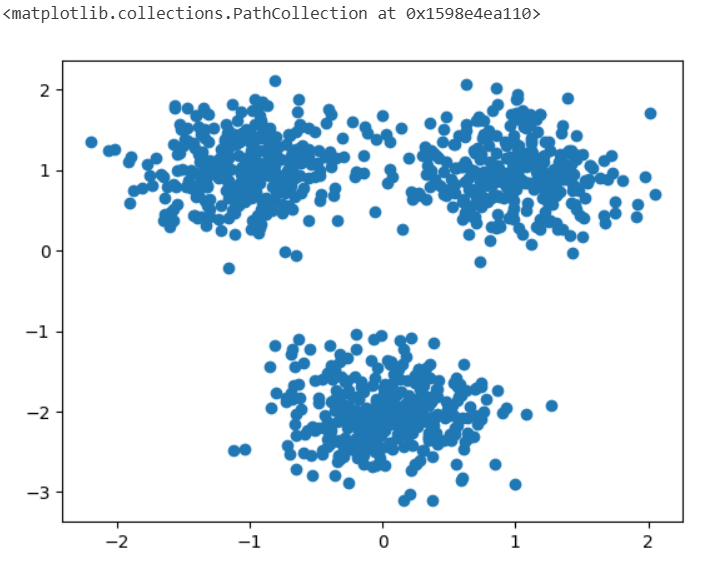
\includegraphics[scale=0.5]{img/205-1}

Приклад виконання алгоритму k-середніх на даному датасеті дано нижче. Тут параметром \verb|n_clusters| передається кількість кластерів, на які потрібно розбити наші дані.

\begin{lstlisting}
import numpy as np
import matplotlib.pyplot as plt
from sklearn.cluster import KMeans

kmeans = KMeans(n_clusters=3, random_state=42)
labels = kmeans.fit_predict(X)
centers = kmeans.cluster_centers_

plt.figure(figsize=(8, 5))
plt.scatter(X[:, 0], X[:, 1], c=labels, cmap='viridis', s=60, edgecolors='k', alpha=0.7)
plt.scatter(centers[:, 0], centers[:, 1], c='red', s=200, marker='X', label='Centroids')
plt.title('K-Means Clustering Example')
plt.xlabel('Feature 1')
plt.ylabel('Feature 2')
plt.legend()
plt.grid(True)
plt.show()
\end{lstlisting}

Результат:

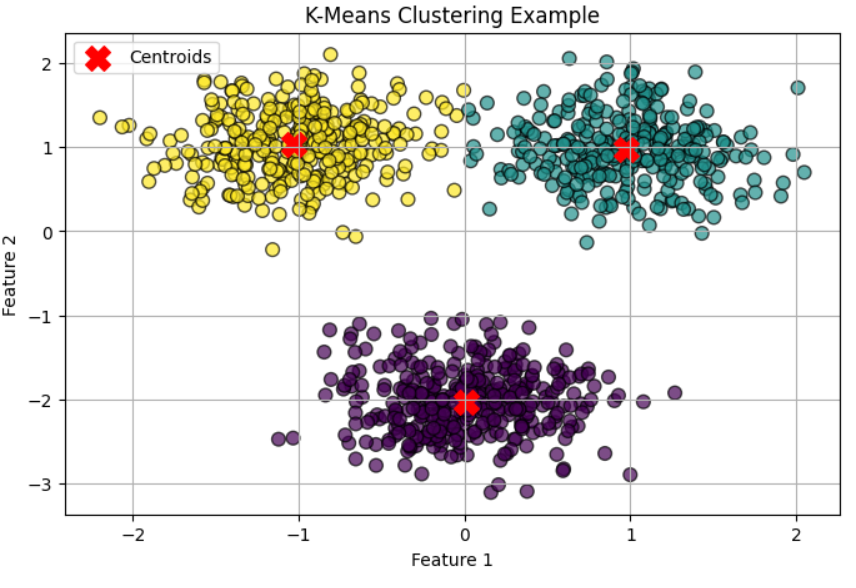
\includegraphics[scale=0.5]{img/205-2}

Алгоритм k-середніх найкраще працює з числовими даними, для яких можна обчислити відстань між об'єктами. Найчастіше використовується евклідова відстань, тому ознаки повинні мати числові значення.

Варто пам'ятати за деякі недоліки цього алгоритму. Результат кластеризації чутливий до початкового вибору центроїдів. Окрім того, метод погано працює з кластерами складної форми.


\subsection{Вибір k: метод ліктя.}

Але яким чином обрати кількість кластерів k?

Метод ліктя — це графічний спосіб вибору оптимальної кількості кластерів.

Для кожного значення $k$ обчислюється сумарна внутрішньокластерна дисперсія (Within Cluster Sum of Squares, WCSS):

$$WCSS=\sum_{i=1}^{k}\sum_{x\in C_i}|x-\mu_i|^2,$$

де $C_i$ — множина об'єктів i-го кластера, $\mu_i$ — центр цього кластера.

Після цього будується графік залежності WCSS від кількості кластерів.

Спочатку зі збільшенням $k$ помилка швидко зменшується, однак після певного моменту покращення стає незначним. Ця точка нагадує вигин ліктя, тому метод і отримав таку назву. Саме відповідне значення $k$ зазвичай вважають оптимальним.


\section{Метод головних компонент.}

Метод головних компонент (Principal Component Analysis, PCA) — це статистичний метод зменшення розмірності даних.
Його ідея полягає в тому, щоб знайти нову систему координат, де:

\begin{itemize}
\item перша вісь (перша головна компонента) пояснює максимальну дисперсію даних,

\item друга — наступну за величиною дисперсію, і т. д.
Так при збереженні головних компонент ми зберігаємо максимум інформації при мінімумі вимірів.
\end{itemize}

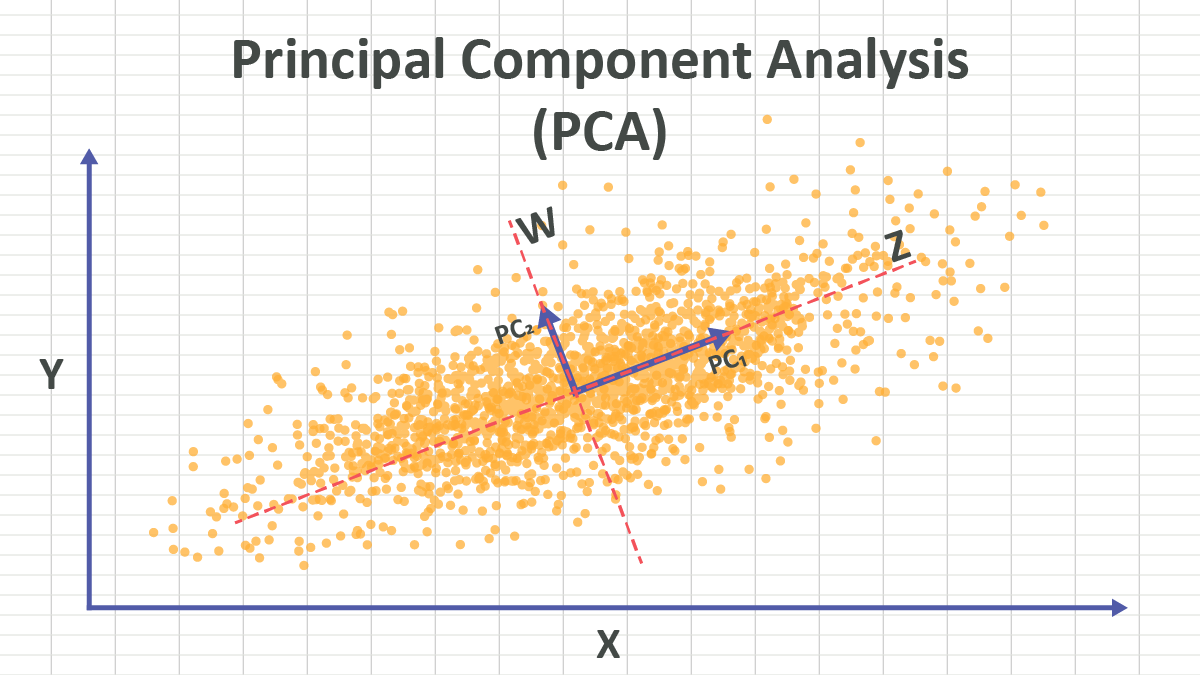
\includegraphics[scale=0.5]{img/ml-uns-2}

Застосуємо алгоритм головних компонент на відомий нам датасет раку молочної залози. Завантажимо дані та виведемо розмірність.

\begin{lstlisting}
import pandas as pd 
import numpy as np 
from sklearn.datasets import load_breast_cancer 

cancer = load_breast_cancer(as_frame=True) 
df = cancer.frame 
print('Original Dataframe shape :',df.shape)
X = df[cancer['feature_names']] 
print('Inputs Dataframe shape :', X.shape)
\end{lstlisting}

Результат:

\begin{console}
Original Dataframe shape : (569, 31)
Inputs Dataframe shape : (569, 30)
\end{console}

30 вхідних ознак потрібно спроектувати на 2 головні ознаки. Нормалізуємо наші дані:

\begin{lstlisting}
X_mean = X.mean()
X_std = X.std()
X_normalized = (X - X_mean) / X_std
\end{lstlisting}

та побудуємо матрицю коваріацій:

\begin{lstlisting}
c = X_normalized.cov() 

import matplotlib.pyplot as plt 
import seaborn as sns 
sns.heatmap(c) 
plt.show()
\end{lstlisting}

Результат:

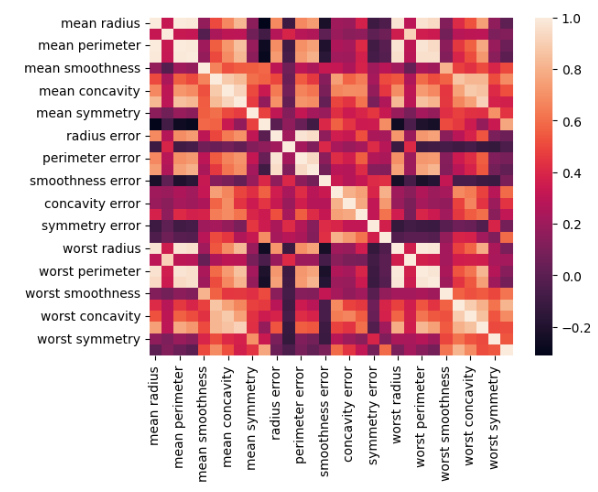
\includegraphics[scale=0.5]{img/205-3}

Знайдемо на основі даних про коваріацію власні значення - власні значення матриці коваріації.

\begin{lstlisting}
eigenvalues, eigenvectors = np.linalg.eig(c) 
print('Eigen values:\n', eigenvalues) 
print('Eigen values Shape:', eigenvalues.shape) 
print('Eigen Vector Shape:', eigenvectors.shape)
\end{lstlisting}

Результат:

\begin{console}
Eigen values:
 [1.32816077e+01 5.69135461e+00 2.81794898e+00 1.98064047e+00
 1.64873055e+00 1.20735661e+00 6.75220114e-01 4.76617140e-01
 4.16894812e-01 3.50693457e-01 2.93915696e-01 2.61161370e-01
 2.41357496e-01 1.57009724e-01 9.41349650e-02 7.98628010e-02
 5.93990378e-02 5.26187835e-02 4.94775918e-02 1.33044823e-04
 7.48803097e-04 1.58933787e-03 6.90046388e-03 8.17763986e-03
 1.54812714e-02 1.80550070e-02 2.43408378e-02 2.74394025e-02
 3.11594025e-02 2.99728939e-02]
Eigen values Shape: (30,)
Eigen Vector Shape: (30, 30)
\end{console}

Проіндексуємо власні значення в порядку спадання, відповідно відсортуємо і власні вектори:

\begin{lstlisting}
idx = eigenvalues.argsort()[::-1] 
eigenvalues = eigenvalues[idx] 
eigenvectors = eigenvectors[:,idx]

explained_var = np.cumsum(eigenvalues) / np.sum(eigenvalues) 
print(explained_var)
\end{lstlisting}

Результат:

\begin{console}
[0.44272026 0.63243208 0.72636371 0.79238506 0.84734274 0.88758796
 0.9100953  0.92598254 0.93987903 0.95156881 0.961366   0.97007138
 0.97811663 0.98335029 0.98648812 0.98915022 0.99113018 0.99288414
 0.9945334  0.99557204 0.99657114 0.99748579 0.99829715 0.99889898
 0.99941502 0.99968761 0.99991763 0.99997061 0.99999557 1.        ]
\end{console}

Визначимо, скільки компонент ми можемо залишити з достатньо великою варіацією (разом ці компоненти мають пояснювати щонайменше 50$\%$ варіації):

\begin{lstlisting}
n_components = np.argmax(explained_var >= 0.50) + 1 
print(n_components)
\end{lstlisting}

Результат:

\begin{console}
2
\end{console}

Побужуємо теплову карту:

\begin{lstlisting}
# PCA components
u = eigenvectors[:,:n_components] 
pca_component = pd.DataFrame(u, index = cancer['feature_names'], columns = ['PC1','PC2'] ) 

plt.figure(figsize =(5, 7)) 
sns.heatmap(pca_component) 
plt.title('PCA Component') 
plt.show()
\end{lstlisting}

Результат:

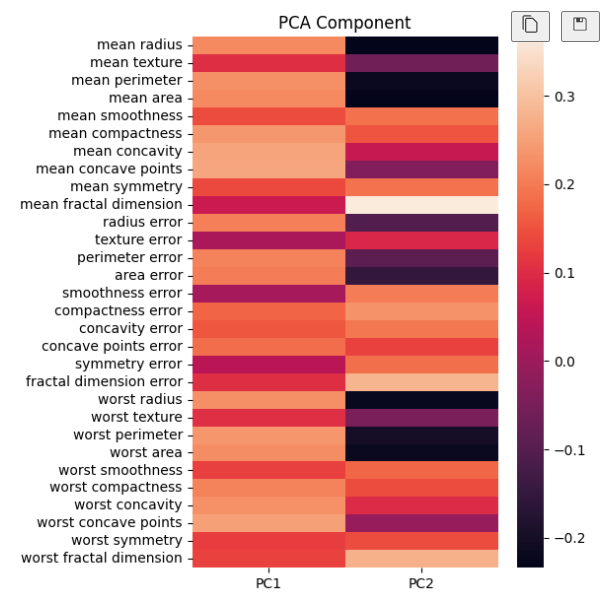
\includegraphics[scale=0.5]{img/205-4}

Множимо матриці нормалізованих даних на PCA компоненти:

\begin{lstlisting}
Z_pca = X_normalized @ pca_component 
Z_pca.rename({'PC1': 'PCA1', 'PC2': 'PCA2'}, axis=1, inplace=True) 
print(Z_pca)
\end{lstlisting}

Результат:

\begin{console}
          PCA1       PCA2
0     9.184755   1.946870
1     2.385703  -3.764859
2     5.728855  -1.074229
3     7.116691  10.266556
4     3.931842  -1.946359
..         ...        ...
564   6.433655  -3.573673
565   3.790048  -3.580897
566   1.255075  -1.900624
567  10.365673   1.670540
568  -5.470430  -0.670047

[569 rows x 2 columns]
\end{console}


Тепер той же самий алгоритм, але використовуємо модуль sklearn.

\begin{lstlisting}
from sklearn.decomposition import PCA

pca = PCA(n_components=2)
pca.fit(X_normalized)
x_pca = pca.transform(X_normalized)

df_pca1 = pd.DataFrame(x_pca, columns=['PC{}'. format(i+1) for i in range(n_components)]) 
print(df_pca1)

plt.figure(figsize=(8, 6)) 
plt.scatter(x_pca[:, 0], x_pca[:, 1], c=cancer['target'], cmap='plasma') 
plt.xlabel('First Principal Component') 
plt.ylabel('Second Principal Component') 
plt.show()
\end{lstlisting}

Результат:

\begin{console}
           PC1        PC2
0     9.184755   1.946870
1     2.385703  -3.764859
2     5.728855  -1.074229
3     7.116691  10.266556
4     3.931842  -1.946359
..         ...        ...
564   6.433655  -3.573673
565   3.790048  -3.580897
566   1.255075  -1.900624
567  10.365673   1.670540
568  -5.470430  -0.670047

[569 rows x 2 columns]
\end{console}

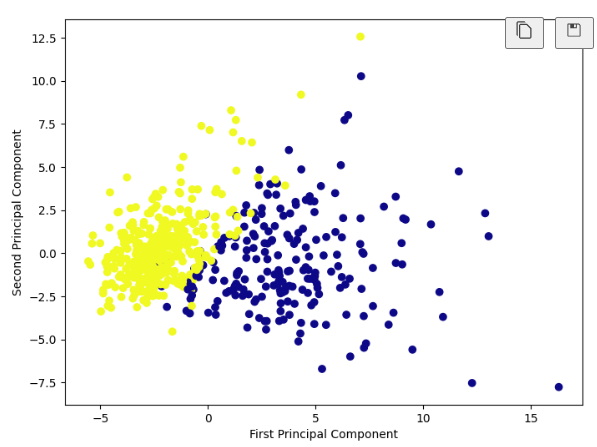
\includegraphics[scale=0.5]{img/205-5}


\ding{46} \textbf{Питання для самоконтролю.}

\begin{enumerate}
\item Що таке навчання без учителя (Unsupervised Learning)?
\item Чим навчання без учителя відрізняється від навчання з учителем?
\item Які основні задачі розв'язуються методами навчання без учителя?
\item У яких сферах застосовується навчання без учителя?
\item Що таке кластеризація?
\item Яка основна ідея алгоритму k-середніх (k-Means)?
\item Як працює алгоритм k-середніх?
\item Що таке центроїд кластера?
\item Як обчислюється центр кластера?
\item Яким чином об'єкти розподіляються між кластерами?
\item Як обирається кількість кластерів k?
\item Що таке метод ліктя (Elbow Method)?
\item Які переваги має алгоритм k-середніх?
\item Які недоліки має алгоритм k-середніх?
\item Як початкове розташування центроїдів впливає на результат кластеризації?
\item Для чого використовується алгоритм k-Means++?
\item Які типи даних найкраще підходять для алгоритму k-середніх?
\item Що таке зменшення розмірності (Dimensionality Reduction)?
\item Для чого застосовується метод головних компонент (PCA)?
\item Яка основна ідея методу головних компонент?
\item Що таке головна компонента?
\item Чому головні компоненти є взаємно ортогональними?
\item Що таке дисперсія ознак і чому вона важлива в PCA?
\item Як PCA дозволяє зменшити кількість ознак без значної втрати інформації?
\item Що таке пояснена дисперсія (Explained Variance)?
\item Як визначити кількість головних компонент, які слід залишити?
\item Чому перед застосуванням PCA часто виконують стандартизацію даних?
\item Які переваги має використання PCA?
\item Які недоліки має метод головних компонент?
\item Як кластеризація та PCA можуть використовуватися разом під час аналізу даних?
\end{enumerate}
